\subsection{Visualizaciones en la interfaz}

El sistema muestra por pantalla una serie de visualizaciones una vez se separa una mezcla con el objetivo de proporcionar inspección visual de los resultados:

\subsubsection{\textit{Waveforms}}
Una vez se separa una mezcla, se presenta por pantalla la forma de onda de cada una de las fuentes y de la mezcla. Ver Figura \ref{fig:waveform-gui}

\begin{figure}[H]
    \begin{center}
    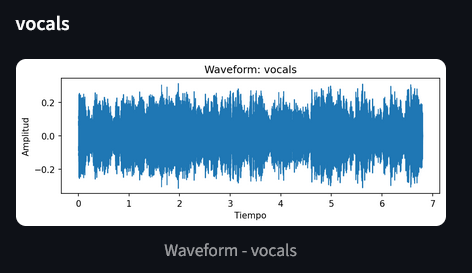
\includegraphics[width=0.7\textwidth]{commons/Waveform_GUI.png}
    \caption{Ejemplo de una forma de onda mostrada en la interfaz al finalizar la separación de una pista.}
    \label{fig:waveform-gui}
    \end{center}
\end{figure}

\subsubsection{Espectrogramas}
A la vez que se muestra la forma de onda de la mezcla y de cada fuente, se muestra en conjunto el respectivo espectrograma. Ver figura \ref{fig:spectrogram-gui}

\begin{figure}[H]
    \begin{center}
    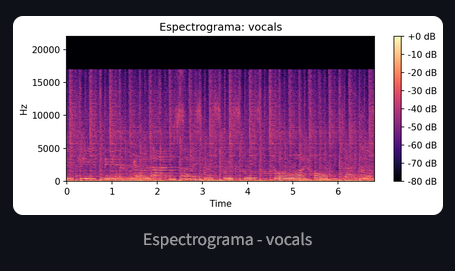
\includegraphics[width=0.7\textwidth]{commons/Espectrograma_GUI.png}
    \caption{Ejemplo de un espectrograma mostrado en la interfaz al finalizar la separación de una pista.}
    \label{fig:spectrogram-gui}
    \end{center}
\end{figure}

